\subsection{Clinical stratification} \label{clin}
The age-stratified late exposed/incubation and both the early and late active disease compartments were further stratified into five ``clinical" categories: \textit{1)} asymptomatic, \textit{2)} symptomatic ambulatory, never detected, \textit{3)} symptomatic ambulatory, ever detected, \textit{4)} ever hospitalised, never critical, and \textit{5)} ever critically unwell (Figure \ref{fig:clinical_strat}).
The proportion of new infectious persons entering stratum 1 (asymptomatic) is age-dependent and constant over time. The proportion of symptomatic patients (strata 2 to 5) ever detected (strata 3 to 5) is set through a parameter that represents the time-varying proportion of all symptomatic patients who are ever detected (the case detection rate). Of those ever symptomatic (strata 2 to 5), an age-specific proportion is considered to be hospitalised (entering strata 4 or 5, constant over time). Of those hospitalised (entering strata 4 or 5), a fixed proportion was considered to be critically unwell (entering stratum 5, Figure \ref{fig:clinical_rationale}, not age-specific, constant over time).

\begin{figure}[ht]
    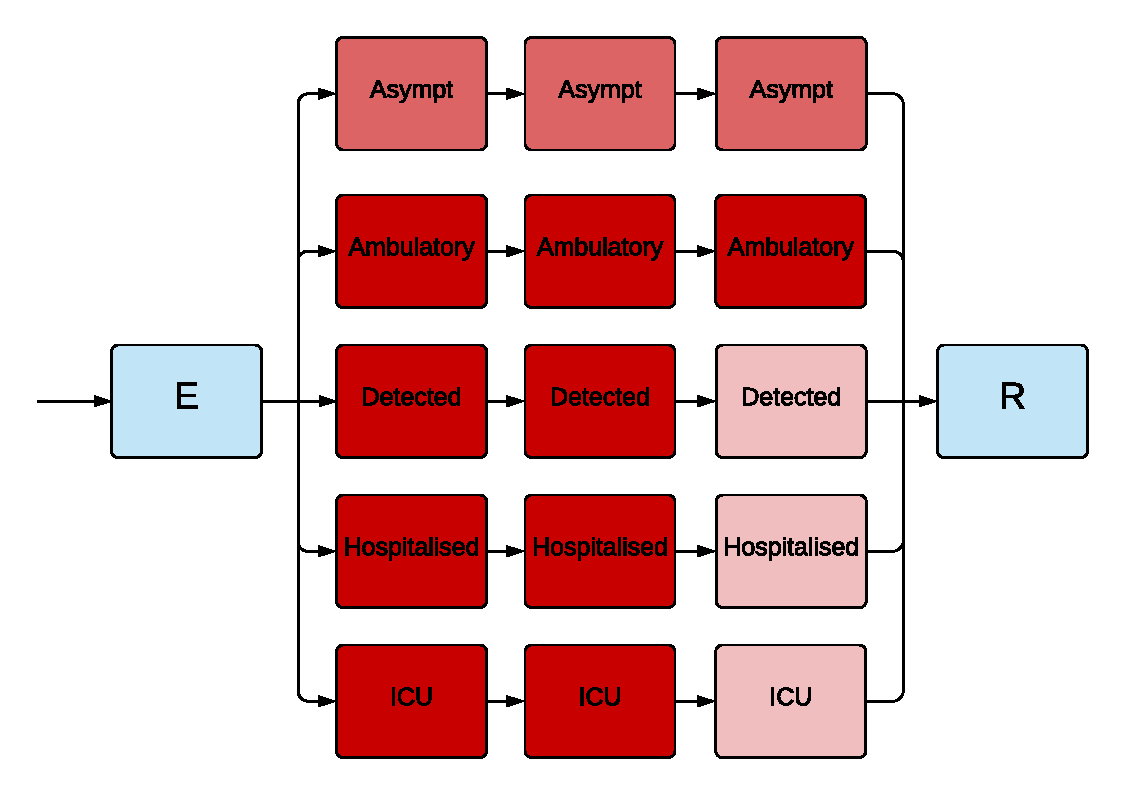
\includegraphics[width=\textwidth]{../covid_19/stratifications/covid_19_clinical_strat.pdf}
    \title{Illustration of the implementation of the clinical stratification.}
    \caption{\textbf{Illustration of the implementation of the clinical stratification.} Depth of pink/red shading indicates the infectiousness of the compartment. Typical parameter values represented, although the infectiousness of asymptomatic persons is varied in calibration.}
    \label{fig:clinical_strat}
\end{figure}

\begin{figure}[ht]
    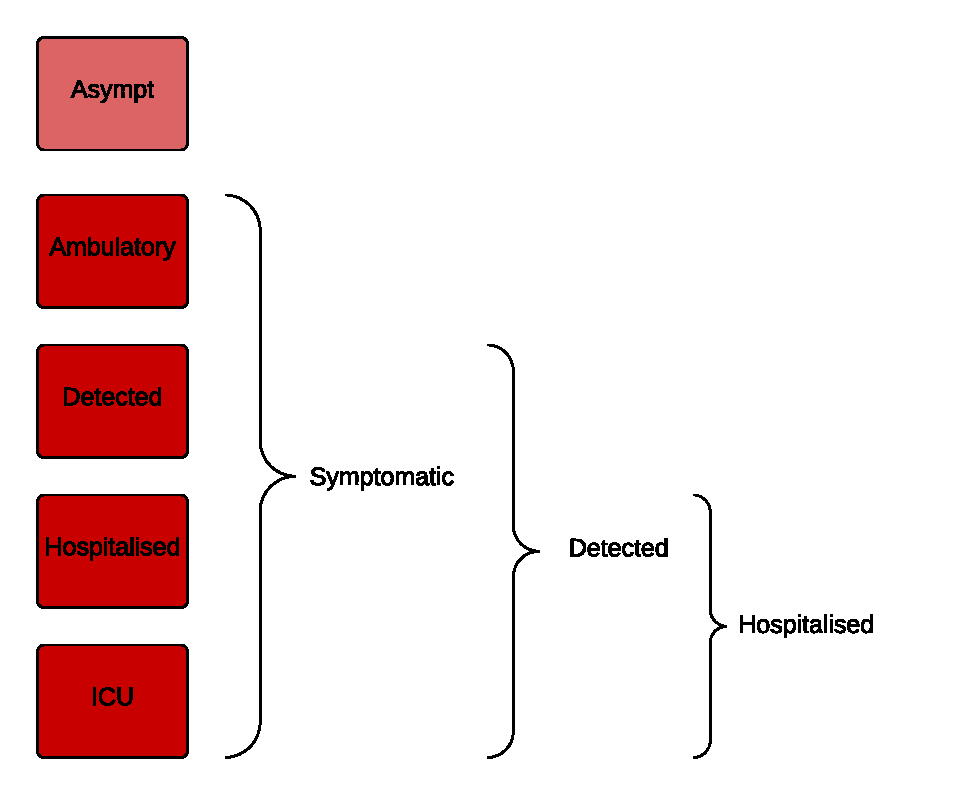
\includegraphics[width=\textwidth]{../covid_19/stratifications/covid_19_clinical_rationale.pdf}
    \title{Illustration of the rationale for the clinical stratification.}
	\caption{\textbf{Illustration of the rationale for the clinical stratification.}}
    \label{fig:clinical_rationale}
\end{figure}

\subsection{Hospitalisation} \label{hosp}
For COVID-19 patients who are admitted to hospital, the sojourn time in the early and late active compartments is modified, superseding the default values of the sojourn times for these compartments. The point of admission to hospital is considered to be the transition from early to late active disease, such that the sojourn time in the late disease represents the period of time admitted to hospital. For patients admitted to ICU, admission to ICU occurs at this same transition point. For this group, the period of time hospitalised prior to ICU admission is estimated as a proportion of the early active period, such that the early active period represents both the period ambulatory in the community and the period in hospital prior to ICU admission.

\subsection{Infectiousness} \label{infect}
Asymptomatic persons are assumed to be less infectious per unit time active than symptomatic persons not undergoing case isolation (typically by around 50\%, although this is varied in calibration/uncertainty analysis). Infectiousness is also decreased for persons who have been detected to reflect case isolation, and for those admitted to hospital or ICU to reflect infection control procedures (by 80\% for all groups, parameter value consistent with typically used modelled values but not informed by empiric estimates). Presymptomatic individuals are assumed to have equivalent infectiousness to those with early active COVID-19.

\subsection{Application of COVID-19-related death}
Age-specific infection fatality rates (IFRs) were applied and distributed across strata 4 and 5, with no deaths typically applied to the first three strata. A ceiling of 50\% is set on the proportion of those admitted to ICU (entering stratum 5) who die. If the infection fatality rate is greater than this ceiling, the proportion of critically unwell persons dying was set to 50\%, with the remainder of the infection fatality rate then applied to the hospitalised proportion. Otherwise, if the infection fatality rate is less than half of the absolute proportion of persons critically unwell, the infection fatality rate is applied entirely through stratum 5 (such that the proportion of critically unwell persons dying in that age group becomes \textless 50\% and the proportion of stratum 4 dying is set to zero). In the event that the infection fatality rate for an age group is greater than the total proportion hospitalised (which is unusual, but could occur for the oldest age group under certain parameter configurations), the remaining deaths are assigned to the asymptomatic stratum. This approach was adopted for computational ease and is valid because the duration active for persons entering this stratum is the same as for the other non-hospitalised strata, such that the dynamics are identical to assigning the deaths to any of the first three strata. We used the age-specific IFRs previously estimated from age-specific death data from 45 countries and results from national-level seroprevalence surveys \cite{RN6}.

\begin{table}[ht]
\renewcommand{\baselinestretch}{1}
    \begin{tabular}{| p{2cm} | p{6.6cm} | p{2.5cm} | l | l |}
    	\hline
        \textbf{Clinical stratum} & \textbf{Stratum name} & \textbf{Pre-symptomatic} &\textbf{Early} & \textbf{Late}\\
        \hline
        1 & Asymptomatic & \cellcolor[HTML]{DC6464}\textcolor[HTML]{FFFFFF}{0.5} & 
        \cellcolor[HTML]{DC6464}\textcolor[HTML]{FFFFFF}{0.5} & \cellcolor[HTML]{DC6464}\textcolor[HTML]{FFFFFF}{0.5} \\
        2 & Symptomatic ambulatory never detected & \cellcolor[HTML]{C90000}\textcolor[HTML]{FFFFFF}{1} & \cellcolor[HTML]{C90000}\textcolor[HTML]{FFFFFF}{1} & \cellcolor[HTML]{C90000}\textcolor[HTML]{FFFFFF}{1} \\
        3 & Symptomatic ambulatory ever detected & \cellcolor[HTML]{C90000}\textcolor[HTML]{FFFFFF}{1} & \cellcolor[HTML]{C90000}\textcolor[HTML]{FFFFFF}{1} & \cellcolor[HTML]{F0BEBE}\textcolor[HTML]{FFFFFF}{0.2} \\
        4 & Hospitalised never critical & \cellcolor[HTML]{C90000}\textcolor[HTML]{FFFFFF}{1} & \cellcolor[HTML]{C90000}\textcolor[HTML]{FFFFFF}{1} & \cellcolor[HTML]{F0BEBE}\textcolor[HTML]{FFFFFF}{0.2} \\
        5 & Ever critically unwell & 
        \cellcolor[HTML]{C90000}\textcolor[HTML]{FFFFFF}{1} & \cellcolor[HTML]{C90000}\textcolor[HTML]{FFFFFF}{1} & \cellcolor[HTML]{F0BEBE}\textcolor[HTML]{FFFFFF}{0.2} \\
        \hline
    \end{tabular}
    	\title{Illustration of the relative infectiousness of disease compartments by clinical stratification and stage of infection.}
    \caption{\textbf{Illustration of the relative infectiousness of disease compartments by clinical stratification and stage of infection.} Typical parameter values displayed.}
    \label{tab:clinical}
\end{table}
